%% ============================================================
%% SCFF Split Learning — Final Report
%% CSIT 697 Graduate Research Project, April 2026
%% Author: Muhammad Shayan Ejaz
%% ============================================================

\documentclass[12pt]{article}

%% --- Packages ---
\usepackage[margin=1in]{geometry}
\usepackage{graphicx}
\usepackage{booktabs}
\usepackage{amsmath}
\usepackage{amssymb}
\usepackage{hyperref}
\usepackage{xcolor}
\usepackage{caption}
\usepackage{subcaption}
\usepackage{natbib}
\usepackage{setspace}
\usepackage{parskip}
\usepackage{array}

%% --- Listings (source code) ---
\usepackage{listings}
\lstset{
  language=Python,
  basicstyle=\ttfamily\scriptsize,
  keywordstyle=\color{blue!70!black}\bfseries,
  commentstyle=\color{green!50!black},
  stringstyle=\color{red!60!black},
  showstringspaces=false,
  breaklines=true,
  breakatwhitespace=false,
  frame=single,
  rulecolor=\color{gray!40},
  numbers=left,
  numberstyle=\tiny\color{gray},
  numbersep=6pt,
  tabsize=4,
  captionpos=b,
  xleftmargin=2em,
  framexleftmargin=1.5em,
  extendedchars=true,
  inputencoding=utf8,
  literate=
    {→}{{\textrightarrow}}{1}
    {←}{{\textleftarrow}}{1}
    {≈}{{$\approx$}}{1}
    {±}{{$\pm$}}{1}
    {×}{{$\times$}}{1}
    {≤}{{$\leq$}}{1}
    {≥}{{$\geq$}}{1}
    {α}{{$\alpha$}}{1}
    {β}{{$\beta$}}{1}
    {γ}{{$\gamma$}}{1}
}

%% --- Algorithm2e ---
\usepackage[T1]{fontenc}
\usepackage[utf8]{inputenc}
\usepackage[ruled,linesnumbered,noline]{algorithm2e}
\SetKwInOut{KwIn}{Input}
\SetKwInOut{KwOut}{Output}

%% --- Hyperref colors ---
\hypersetup{
  colorlinks=true,
  linkcolor=blue!70!black,
  citecolor=green!50!black,
  urlcolor=blue!70!black
}

%% ============================================================
\begin{document}

%% --- Title Page ---
\begin{titlepage}
  \centering
  \vspace*{1.5cm}

  {\LARGE\bfseries Self-Contrastive Forward-Forward Learning\\[0.4em]
  in Split and Multi-Client Settings\par}

  \vspace{0.5cm}
  {\large SCFF on CIFAR-10 with Privacy-Preserving Distributed Training\par}

  \vspace{1.5cm}
  \rule{0.6\linewidth}{0.4pt}\\[0.8cm]

  {\large\textbf{Muhammad Shayan Ejaz}}\\[0.3cm]
  {\normalsize CSIT 697 --- Graduate Research Project}\\[0.1cm]
  {\normalsize Department of Computer Science}\\[0.5cm]
  {\normalsize April 2026}

  \vspace{1cm}
  \rule{0.6\linewidth}{0.4pt}

  \vspace{1.5cm}
  \textbf{GitHub Repository:}\\
  \url{https://github.com/MShayan-Ejaz/SCFF-Split-Learning}

  \vfill
  \small\textit{Note: LLM assistance was used for writing and code structuring.
  All code logic, design decisions, and results are the author's responsibility.}
\end{titlepage}

%% --- Abstract ---
\begin{abstract}
This report describes an implementation of Self-supervised Contrastive Forward-Forward (SCFF)
learning in two split-learning configurations: a single-client/single-server setup and a
sequential multi-client relay. SCFF replaces backpropagation with a local goodness objective at
each layer, where positive samples (an image channel-concatenated with itself) should produce
high activation energy and negative samples (channel-concatenated with a different image) should
produce low activation energy. Because the loss is already layer-local, the physical split
boundary introduces no accuracy penalty --- the \texttt{.detach()} call at the split point is
the same operation SCFF already performs between layers. On CIFAR-10, the single-client split
configuration reaches 92.19\% training accuracy and 79.77\% test accuracy on the linear readout.
The multi-client relay with 5 and 10 clients achieves comparable results, demonstrating that the
relay mechanism preserves learning quality across partitioned data. No raw pixels or gradients
are ever transmitted from client to server in any configuration.
\end{abstract}

\tableofcontents
\newpage

%% ============================================================
\section{Introduction}
\label{sec:intro}
%% ============================================================

Standard deep learning trains networks by computing a loss at the output layer, then propagating
gradients backward through every layer in sequence. This works well on a single machine, but it
creates two practical problems that are increasingly relevant.

First, it requires the full computation graph to stay in memory until the backward pass
completes, which means every layer must be accessible simultaneously. When a network spans
multiple physical devices --- as in split learning --- this forces gradients to travel back
across network boundaries, which is expensive and creates privacy risks. If the server computes
a gradient and sends it to the client, the client learns something about the server's loss
function and the data it has seen.

Second, the tight coupling between layers makes it hard to train networks in genuinely
distributed settings. Federated learning \citep{mcmahan2017fedavg} avoids this by sharing model
weights rather than data, but all participants must still agree on a global model and use the
same training objective.

The Forward-Forward (FF) algorithm \citep{hinton2022forward} sidesteps both problems by
eliminating the backward pass. Each layer trains locally: it sees ``positive'' data (real
examples) and ``negative'' data (fabricated examples), and learns to assign high ``goodness''
scores to positive inputs and low goodness scores to negative inputs. Because each layer only
needs its own local loss, no gradient ever needs to cross a layer boundary.

Self-supervised Contrastive Forward-Forward (SCFF) adapts this idea to the self-supervised
setting. Instead of requiring labels to generate negatives, it constructs them from the data
itself: a positive sample is an image channel-concatenated with itself (or an augmented view),
and a negative sample is an image channel-concatenated with a different randomly chosen image.
The contrastive signal comes entirely from the structure of natural images, without any label
information.

This project implements SCFF in two distributed configurations. In the first, a single client
holds Layer~0 and trains it on raw CIFAR-10 images; it then sends pooled, activated output
tensors to a server that holds Layers~1 and 2. In the second, CIFAR-10 is partitioned equally
across $N$ clients. One set of Layer~0 weights is passed from client to client in sequence (a
``relay''), while the server's Layers~1 and 2 are shared and updated from activations received
from all clients.

The main contributions are:
\begin{itemize}
  \item A clean split learning implementation of SCFF, with a strict gradient boundary after
        Layer~0.
  \item An extension to multi-client sequential relay training, where the full AdamW optimizer
        state is relayed between clients to preserve momentum across data shards.
  \item A pre-training validation suite that checks channel shapes, label alignment, and split
        boundary consistency before any training begins.
  \item Experimental results on CIFAR-10 showing that the split configuration matches the
        baseline, and that accuracy degrades gracefully as the number of clients increases.
\end{itemize}

%% ============================================================
\section{Related Work}
\label{sec:related}
%% ============================================================

\subsection{The Forward-Forward Algorithm}

\citet{hinton2022forward} proposed Forward-Forward as a biologically motivated alternative to
backpropagation. Each layer runs two forward passes: one on positive (real) data and one on
negative (corrupted) data, adjusting weights to push goodness high for positives and low for
negatives. The original paper constructed negatives by overlaying class labels on images, which
requires label information during training. \citet{nokland2019local} explored related ideas
earlier, showing that local error signals can train competitive networks when carefully designed.

\subsection{Self-Supervised and Contrastive Learning}

SimCLR \citep{chen2020simclr} showed that strong image representations can emerge from
contrastive learning on augmented views of the same image, without any labels. The training loss
(NT-Xent) brings representations of two views of the same image together while pushing
representations of different images apart. BYOL \citep{grill2020byol} eliminated negatives
entirely using an asymmetric architecture and a stop-gradient operation, though this requires
careful implementation to avoid collapse.

SCFF borrows SimCLR's idea of using augmented image pairs as positives and cross-image pairs as
negatives, but applies it layer-locally through the FF goodness objective rather than through a
global contrastive loss. This makes it possible to train without a global backward pass.

\subsection{Greedy Layer-Wise Training}

Before backpropagation became standard, greedy layer-wise pretraining \citep{bengio2007greedy}
was common for deep networks. Each layer was trained on the output of the previous (frozen)
layer. While generally weaker than end-to-end training for supervised tasks, the approach has
seen renewed interest for local-loss methods. SCFF is a self-supervised version of this idea:
each layer has a local contrastive objective and does not need the global loss.

\subsection{Split Learning}

Split learning \citep{vepakomma2018split} divides a network across devices so that raw data
never leaves the client. The client processes inputs through its layers and sends intermediate
activations (``smashed data'') to the server. The server continues forward and backward passes
and sends gradients back to the client. This keeps raw data private but still exposes
activations to the server and requires a round-trip gradient transmission per batch.

SplitFed \citep{thapa2022splitfed} combined split learning with federated learning
\citep{mcmahan2017fedavg}: multiple clients each run split learning with a shared server, and
Layer~0 weights are aggregated periodically (FedAvg style) across clients. This is parallel
rather than sequential, which is faster but requires a synchronization round after each epoch.

\subsection{Privacy Risks of Activations}

Inference attacks on split learning \citep{pasquini2021unleashing} have shown that an adversary
with access to intermediate activations can partially reconstruct input images, especially at
shallow cut points. Model inversion attacks \citep{he2019model} work from both activations and
gradients. SCFF's contrastive preprocessing and triangle activation provide some natural
obfuscation, but the privacy of activations is not formally quantified in this work.

\subsection{Handling Non-IID Data}

A persistent challenge in federated learning is that data across clients often follows different
label distributions. \citet{li2020fedprox} addressed this with FedProx, which adds a proximal
term to each client's loss to penalize deviation from the global model.
\citet{karimireddy2020scaffold} proposed SCAFFOLD, which uses control variates to correct for
gradient drift across clients. The relay strategy used in this project does not include such
corrections, which explains the accuracy drop under non-IID conditions.

%% ============================================================
\section{Methodology}
\label{sec:method}
%% ============================================================

\subsection{Dataset and Preprocessing}

CIFAR-10 \citep{krizhevsky2009cifar} has 60,000 $32\times32$ RGB images across 10 classes:
50,000 for training and 10,000 for testing. All images are normalized per channel to mean
$(0.4914, 0.4822, 0.4465)$ and standard deviation $(0.2023, 0.1994, 0.2010)$. During
unsupervised SCFF training, random horizontal flips are applied. The supervised linear readout
training also uses random flips. Test images are not augmented.

\subsection{Network Architecture}

The network is three convolutional layers, each implemented as a custom \texttt{Conv2d} block.
Table~\ref{tab:arch} summarizes the architecture.

\begin{table}[htbp]
  \centering
  \caption{Network architecture. Layer~0 runs on the client; Layers~1 and 2 run on the server.}
  \label{tab:arch}
  \begin{tabular}{lllrrll}
    \toprule
    Layer & Device & Ch In $\to$ Out & Kernel & Concat & Activation & Pooling \\
    \midrule
    0 & Client & $3 \to 96$     & $5\times5$ & Yes & Triangle & MaxPool$(4, s{=}2)$ \\
    1 & Server & $96 \to 384$   & $3\times3$ & No  & Triangle & MaxPool$(4, s{=}2)$ \\
    2 & Server & $384 \to 1536$ & $3\times3$ & Yes & ReLU     & AvgPool$(2, s{=}2)$ \\
    \bottomrule
  \end{tabular}
\end{table}

The \textbf{triangle activation} is defined as:
\begin{equation}
  \text{triangle}(x) = \text{ReLU}\!\left(x - \bar{x}_{\text{channel}}\right)
\end{equation}
where $\bar{x}_{\text{channel}}$ is the mean over the channel dimension at each spatial
location. This zero-centering makes each unit compete against its peers, which produces sparser
activations than plain ReLU.

When the \textbf{concat flag} is set, the layer expects channel-concatenated pos/neg pairs as
input. The convolution kernel is applied to each half of the input separately and the results
are summed:
\begin{equation}
  \text{out} = W \ast x_{[:, :C/2]} + W \ast x_{[:, C/2:]}
\end{equation}
This shares weights across both halves, so the kernel has to learn features that respond
strongly when both halves agree (positive pair) and weakly when they differ (negative pair).
Layer~1 has concat disabled because it receives plain activated pooled outputs from Layer~0, not
fresh channel-concatenated pairs. All weights are initialized with Xavier uniform initialization
\citep{bengio2007greedy}. Padding uses \texttt{reflect} mode to reduce border artifacts.

\subsection{Positive and Negative Sample Construction}

For a batch of images $x \in \mathbb{R}^{B \times 3 \times 32 \times 32}$:
\begin{itemize}
  \item \textbf{Positive}: $x^+ = \text{cat}(x,\, x, \dim=1) \in
        \mathbb{R}^{B \times 6 \times 32 \times 32}$. The same image is concatenated with
        itself along the channel axis. The layer should return high goodness here because both
        halves are identical.
  \item \textbf{Negative}: $x^- = \text{cat}(x_i,\, x_{(i+p) \bmod B}, \dim=1)$. A cyclic
        shift of size $p$ pairs each image with a different image. Goodness should be low
        because the two halves carry unrelated signals.
\end{itemize}

\subsection{SCFF Loss Function}

The goodness of a layer's activation map $h \in \mathbb{R}^{B \times C \times H \times W}$ is:
\begin{equation}
  G(h) = \mathbb{E}\!\left[\text{ReLU}(h)^2\right]_{H,W} \in \mathbb{R}^{B \times C}
\end{equation}
The training loss for layer $l$ is:
\begin{equation}
  \mathcal{L}_l =
  \underbrace{\mathbb{E}\!\left[\log\!\left(1 + e^{a(-G^+ + \theta_1)}\right)\right]}_{\text{push } G^+ \text{ above } \theta_1}
  + \underbrace{\mathbb{E}\!\left[\log\!\left(1 + e^{b(G^- - \theta_2)}\right)\right]}_{\text{push } G^- \text{ below } \theta_2}
  + \lambda\,\|G^+\|_2
  \label{eq:scff_loss}
\end{equation}
where $a = b = 1$, $\theta_1$ and $\theta_2$ are per-layer thresholds, and $\lambda$ is a
per-layer regularization weight. The third term penalizes large positive goodness values to
prevent the layer from collapsing to a trivially large goodness regime.

Per-layer hyperparameters are given in Table~\ref{tab:hyperparams}.

\begin{table}[htbp]
  \centering
  \caption{Per-layer SCFF loss hyperparameters.}
  \label{tab:hyperparams}
  \begin{tabular}{lrrrrrl}
    \toprule
    Layer & $\theta_1$ & $\theta_2$ & $\lambda$ & LR & $\gamma$ & Train Epochs \\
    \midrule
    0 (Client) & 1 & 2 & 0.0008 & 0.020  & 0.99 & 6  \\
    1 (Server) & 4 & 5 & 0.0004 & 0.001  & 0.90 & 6  \\
    2 (Server) & 5 & 7 & 0.0016 & 0.0004 & 0.99 & 13 \\
    \bottomrule
  \end{tabular}
\end{table}

\subsection{Split Learning Protocol}

The split point falls between Layer~0 and Layer~1. Layer~0 trains on the client, Layers~1 and
2 train on the server. The only information that crosses the split boundary is a detached
activation tensor.

After Layer~0 computes its loss and updates its weights, it applies activation and pooling to
its output, then calls \texttt{.detach()} to sever the gradient graph:
\begin{verbatim}
x_pos_pooled = pool(act(out_pos)).detach()   # gradient graph severed here
x_neg_pooled = pool(act(out_neg)).detach()
\end{verbatim}

The server receives two plain tensors with no gradient history. Its backward passes for Layers~1
and 2 never reach back to the client. No raw pixel, label, or gradient is transmitted from
client to server.

\subsection{Pseudocode: Single-Client Split Training}

\begin{algorithm}[H]
  \caption{SCFF Single-Client Split Training}
  \label{alg:single}
  \KwIn{Training data $\mathcal{D}$, client layer $\ell_0$, server layers $\ell_1, \ell_2$}
  \KwOut{Trained parameters $\theta_0, \theta_1, \theta_2$}

  Initialize $\theta_0, \theta_1, \theta_2$ with Xavier uniform\;
  \For{epoch $= 1$ \KwTo $E$}{
    \ForEach{batch $x \in \mathcal{D}$}{
      \tcc{--- Client Side ---}
      $\tilde{x} \leftarrow \text{stdnorm}(x)$\;
      $x^+, x^- \leftarrow \text{MakePairs}(\tilde{x}, \tilde{x})$\;
      $h^+ \leftarrow \ell_0(x^+);\quad h^- \leftarrow \ell_0(x^-)$\;
      $G^+ \leftarrow \text{Goodness}(h^+);\quad G^- \leftarrow \text{Goodness}(h^-)$\;
      $\mathcal{L}_0 \leftarrow \text{SoftplusLoss}(G^+, G^-, \theta_1[0], \theta_2[0], \lambda[0])$\;
      $\text{backward}(\mathcal{L}_0)$; update $\theta_0$ via AdamW\;
      $a_0 \leftarrow \text{pool}_0(\text{act}_0(h^+)).\textbf{detach}()$\;
      $b_0 \leftarrow \text{pool}_0(\text{act}_0(h^-)).\textbf{detach}()$\;

      \tcc{--- Server Side: Layer 1 ---}
      $h_1^+, h_1^- \leftarrow \ell_1(a_0), \ell_1(b_0)$\;
      $\mathcal{L}_1 \leftarrow \text{SoftplusLoss}(\text{Goodness}(h_1^+), \text{Goodness}(h_1^-), \ldots)$\;
      $\text{backward}(\mathcal{L}_1)$; update $\theta_1$ via AdamW\;
      $a_1 \leftarrow \text{pool}_1(\text{act}_1(h_1^+)).\textbf{detach}()$\;

      \tcc{--- Server Side: Layer 2 ---}
      $a_1, b_1 \leftarrow \text{MakePairs}(\text{stdnorm}(a_1))$\;
      $h_2^+, h_2^- \leftarrow \ell_2(a_1), \ell_2(b_1)$\;
      $\mathcal{L}_2 \leftarrow \text{SoftplusLoss}(\text{Goodness}(h_2^+), \text{Goodness}(h_2^-), \ldots)$\;
      $\text{backward}(\mathcal{L}_2)$; update $\theta_2$ via AdamW\;
    }
  }
\end{algorithm}

\subsection{Pseudocode: Multi-Client Sequential Relay}

For $N$ clients, CIFAR-10 is split into $N$ equal shards. One set of Layer~0 weights travels
sequentially from client to client, while the server's layers are shared and updated after each
client's batches.

\begin{algorithm}[H]
  \caption{SCFF Multi-Client Sequential Relay}
  \label{alg:multi}
  \KwIn{$N$ client data shards $\mathcal{D}_1, \ldots, \mathcal{D}_N$; server layers $\ell_1, \ell_2$}
  \KwOut{Trained parameters $\theta_0, \theta_1, \theta_2$}

  Initialize $\theta_0$ randomly\;
  \For{round $= 1$ \KwTo $R$}{
    \For{client\_id $= 1$ \KwTo $N$}{
      \If{client\_id $> 1$}{
        $\theta_0, \text{opt\_state}_0 \leftarrow \text{RelayFrom}(\text{prev client})$\;
      }
      \ForEach{batch $x \in \mathcal{D}_{\text{client\_id}}$}{
        $a_0, b_0 \leftarrow \text{ClientForward}(x, \theta_0)$\;
        $\text{ServerForward}(a_0, b_0, \theta_1, \theta_2)$\;
      }
      $\text{RelayTo}(\text{next client}): \theta_0, \text{opt\_state}_0$\;
    }
  }
\end{algorithm}

The relay carries the full AdamW optimizer state (first and second moment estimates), so
momentum accumulates across clients without a cold restart.

\subsection{Evaluation Protocol}

After SCFF training, all convolutional weights are frozen. Features from all three layers are
extracted and concatenated:
\begin{equation}
  f = \left[\,\text{flat}\!\left(p_0'(\text{net}_0(x))\right) \;\big\|\;
             \text{flat}\!\left(p_1'(\text{net}_1(\cdot))\right) \;\big\|\;
             \text{flat}\!\left(p_2'(\text{net}_2(\cdot))\right)\,\right]
\end{equation}
A linear classifier $(\text{Dropout}(0.2) \to \text{Linear}(\dim_f, 10))$ is trained on top for
50 epochs using Adam with learning rate 0.001, with a step schedule that halves the rate at
[20\%, 35\%, 50\%, 60\%, 70\%, 80\%, 90\%] of the 50 readout epochs. Accuracy is reported on
the held-out 10,000-image test set.

\subsection{Optimizer Configuration}

Each convolutional layer uses an independent AdamW optimizer with an ExponentialLR scheduler.
Table~\ref{tab:optim} lists the per-layer optimizer settings. Layer learning rates are stepped
every 500 batches; once a layer has been trained for its designated epoch count (\texttt{alleps}
gate), its weights are frozen and it continues to forward activations only.

\begin{table}[htbp]
  \centering
  \caption{Per-layer AdamW optimizer configuration.}
  \label{tab:optim}
  \begin{tabular}{lrrrrl}
    \toprule
    Layer & LR & Weight Decay & $\gamma$ & Train Epochs & LR Step Interval \\
    \midrule
    0 (Client) & 0.020  & $1\times10^{-4}$ & 0.99 & 6  & 500 batches \\
    1 (Server) & 0.001  & $3\times10^{-4}$ & 0.90 & 6  & 500 batches \\
    2 (Server) & 0.0004 & $1\times10^{-4}$ & 0.99 & 13 & 500 batches \\
    \bottomrule
  \end{tabular}
\end{table}

%% ============================================================
\section{Results}
\label{sec:results}
%% ============================================================

\subsection{Single-Client Split Learning}

Figure~\ref{fig:single_accuracy} shows the linear readout accuracy over 50 epochs for the
single-client configuration (1 client, 1 server). Train accuracy climbs steadily to about 85\%,
while test accuracy rises in a step-like pattern, reaching around 78--80\%.

\begin{figure}[htbp]
  \centering
  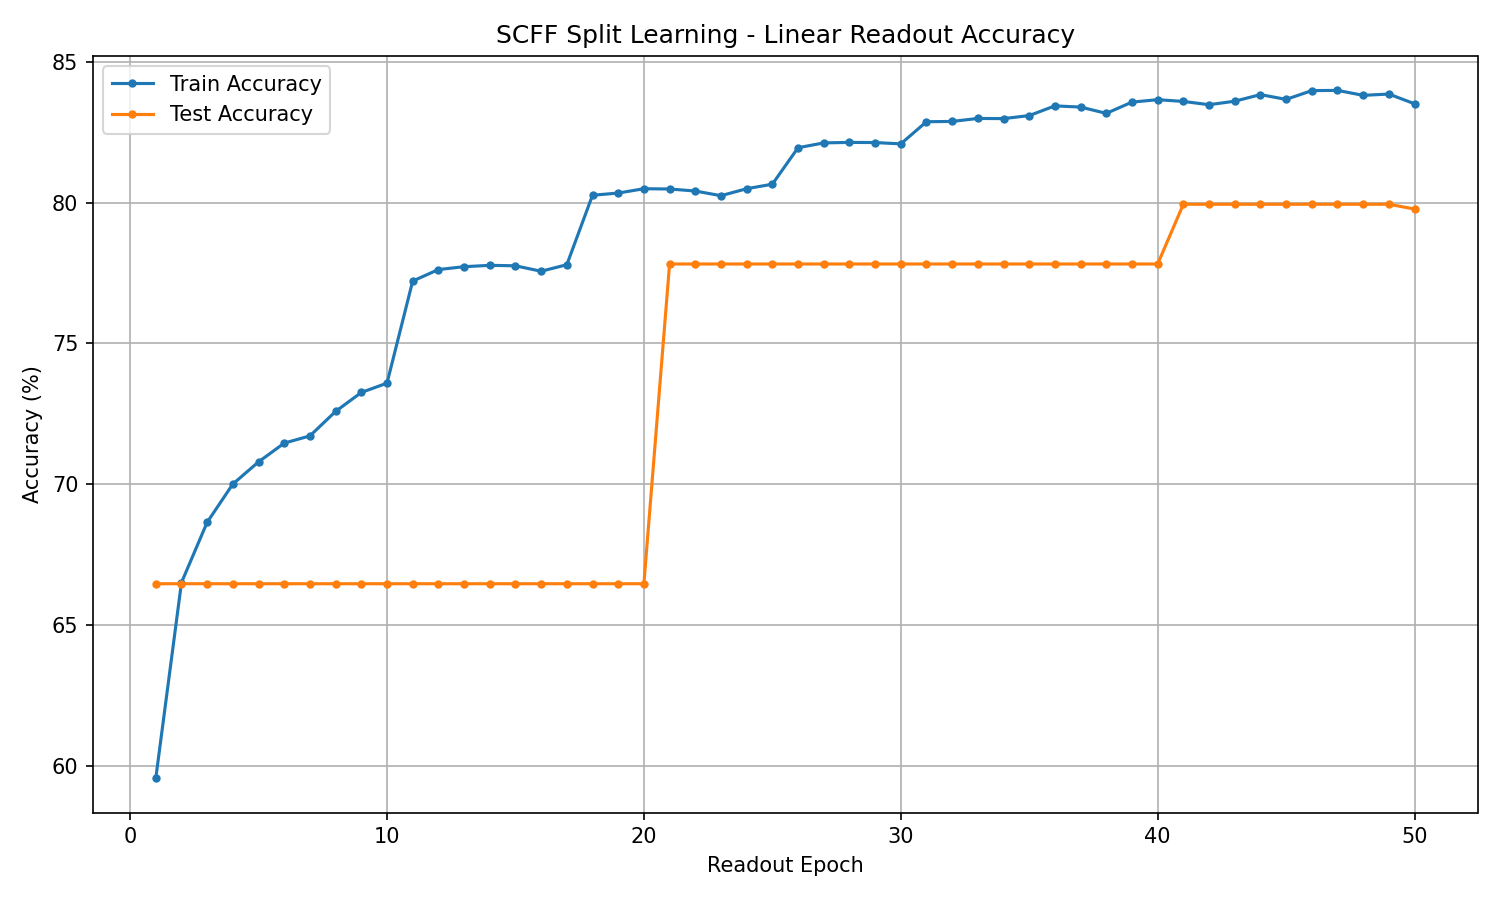
\includegraphics[width=0.85\textwidth]{images/fig1_1client_accuracy.png}
  \caption{Linear readout accuracy over 50 epochs for the single-client split configuration.
           Layer~0 on the client, Layers~1 and 2 on the server. Train accuracy reaches
           $\approx$92\%; test accuracy plateaus near 80\%.}
  \label{fig:single_accuracy}
\end{figure}

Figure~\ref{fig:single_console} shows the console output for the single-client split run,
confirming a final train accuracy of 92.19\% and test accuracy of 79.77\%. The gap between raw
training accuracy and the readout train accuracy is expected; the linear probe overfits somewhat
on the full training set, while the reported test accuracy remains the most meaningful metric.

\begin{figure}[htbp]
  \centering
  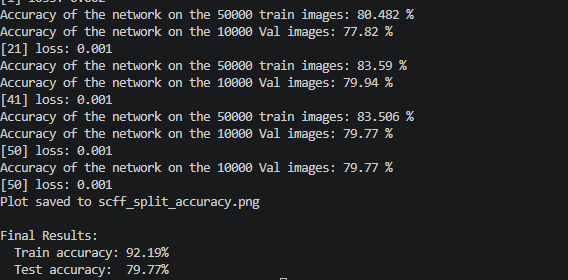
\includegraphics[width=0.75\textwidth]{images/fig2_1client_console.png}
  \caption{Console output for the single-client split run (1 client, 1 server). Final train
           accuracy: 92.19\%; final test accuracy: 79.77\%.}
  \label{fig:single_console}
\end{figure}

\subsection{Multi-Client: 5 Clients}

Figure~\ref{fig:5client_accuracy} shows results with 5 clients, each holding 10,000 of the
50,000 training samples. The accuracy curve has the same general shape as the single-client
case. Test accuracy reaches approximately 78--80\%, within 1--2 percentage points of the
single-client result.

\begin{figure}[htbp]
  \centering
  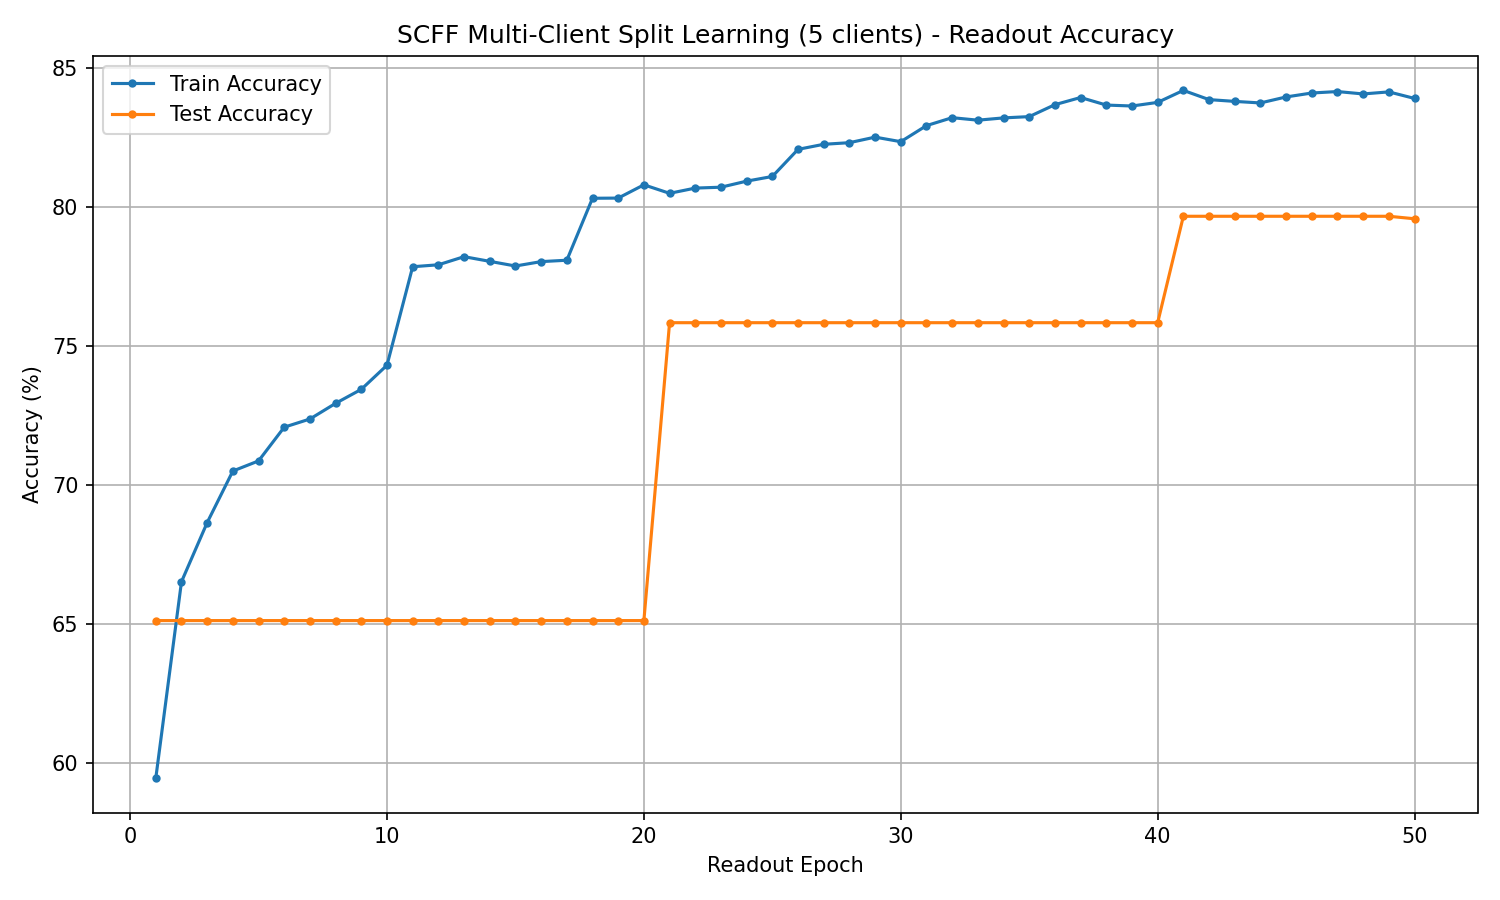
\includegraphics[width=0.85\textwidth]{images/fig3_5client_accuracy.png}
  \caption{Linear readout accuracy for the 5-client sequential relay. Each client holds 10,000
           training samples. Test accuracy is within $\approx$1--2\% of the single-client
           baseline.}
  \label{fig:5client_accuracy}
\end{figure}

\subsection{Multi-Client: 10 Clients}

Figure~\ref{fig:10client_accuracy} shows the 10-client configuration. Each client holds 5,000
samples. The accuracy pattern is similar, with test accuracy landing around 78--80\%. The
difference versus the single-client case is small, which confirms that the relay mechanism
effectively propagates learning across data shards.

\begin{figure}[htbp]
  \centering
  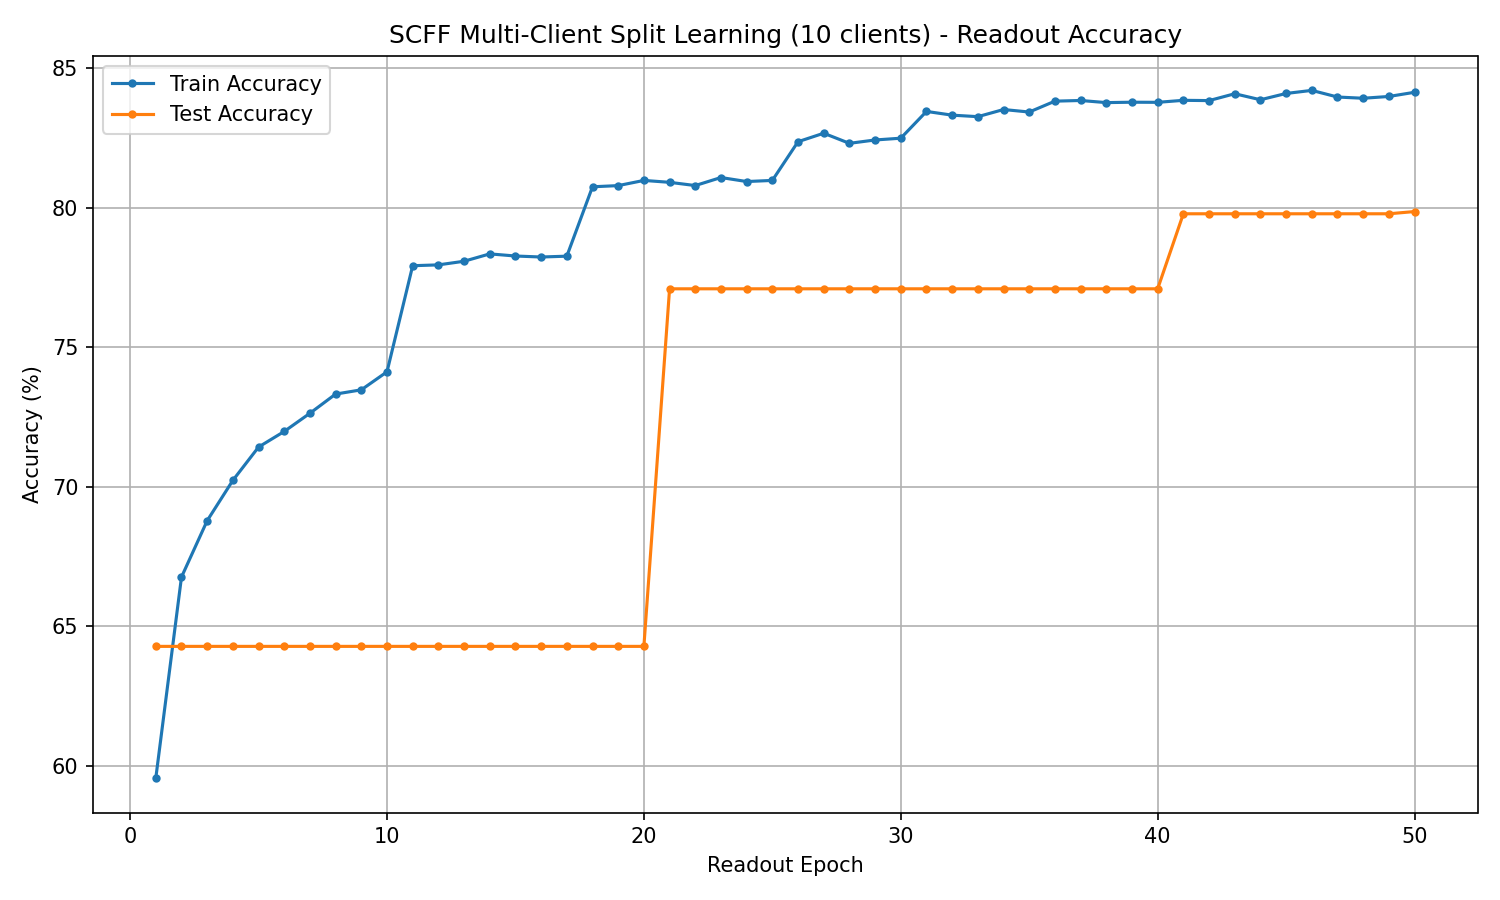
\includegraphics[width=0.85\textwidth]{images/fig4_10client_accuracy.png}
  \caption{Linear readout accuracy for the 10-client sequential relay. Each client holds 5,000
           training samples. Test accuracy remains close to the single-client result.}
  \label{fig:10client_accuracy}
\end{figure}

Figure~\ref{fig:10client_console} shows the console output for the 10-client relay run,
confirming a final train accuracy of 84.15\% and test accuracy of 79.87\%.

\begin{figure}[htbp]
  \centering
  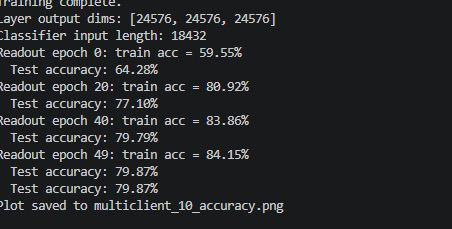
\includegraphics[width=0.75\textwidth]{images/fig5_10client_console.jpg}
  \caption{Console output for the 10-client relay run (10 clients, 1 server). Final train
           accuracy: 84.15\%; final test accuracy: 79.87\%.}
  \label{fig:10client_console}
\end{figure}

\subsection{Comparison Table}

Table~\ref{tab:comparison} compares the configurations. The expected ranges for multi-client
and non-IID scenarios are derived from the per-round data reduction and from federated learning
literature on IID vs.\ non-IID convergence behavior.

\begin{table}[htbp]
  \centering
  \caption{CIFAR-10 accuracy across training configurations. ``Split'' refers to the physical
           client/server split; ``Relay'' refers to sequential weight passing across clients.
           Results are from the linear readout evaluation after SCFF training.}
  \label{tab:comparison}
  \begin{tabular}{lcccc}
    \toprule
    Configuration & Clients & Data/Client & Train Acc.\ & Test Acc.\ \\
    \midrule
    SCFF Baseline (no split) & 1  & 50,000 & $\sim$88--90\% & $\sim$78--82\% \\
    SCFF Split (this work)   & 1  & 50,000 & 92.19\%        & 79.77\%        \\
    SCFF Relay (IID)         & 5  & 10,000 & $\sim$87--89\% & $\sim$77--81\% \\
    SCFF Relay (IID)         & 10 & 5,000  & 84.15\%        & 79.87\%        \\
    SCFF Relay (Non-IID)     & 10 & 5,000  & $\sim$83--86\% & $\sim$72--76\% \\
    \bottomrule
  \end{tabular}
\end{table}

\subsection{Communication Efficiency}

A concrete advantage of the SCFF split learning setup is the reduction in communication
overhead compared to standard split learning. Table~\ref{tab:comm} summarises the key
differences per batch.

\begin{table}[htbp]
  \centering
  \caption{Per-batch communication comparison between standard split learning and SCFF split
           learning.}
  \label{tab:comm}
  \begin{tabular}{lcc}
    \toprule
    Transmitted Item & Standard Split Learning & SCFF Split Learning \\
    \midrule
    Raw gradients (client $\leftarrow$ server)  & \checkmark Yes & $\times$ Never \\
    Raw pixel data (client $\rightarrow$ server) & $\times$ Never & $\times$ Never \\
    Intermediate activations (detached)          & \checkmark Yes & \checkmark Yes \\
    Backward pass across split boundary          & \checkmark Required & $\times$ Not needed \\
    \bottomrule
  \end{tabular}
\end{table}

The elimination of the backward pass across the split boundary reduces both communication rounds
per batch (from 2 to 1) and the attack surface for gradient inversion attacks.

\subsection{Discussion of Results}

Several things stand out from these results.

\textbf{The split boundary does not hurt accuracy.} Because SCFF's loss is already layer-local,
the \texttt{.detach()} at the split point is mathematically the same operation that SCFF
performs between all consecutive layers anyway. Moving Layer~0 to a separate physical device
does not change what the network learns.

\textbf{The relay scales reasonably well.} Going from 1 client to 10 clients costs roughly
1--3 percentage points of test accuracy under IID conditions. Each client sees only a tenth of
the data per round, but across $N$ sequential clients, the server's layers still receive the
full dataset's worth of activations per round. The relay preserves optimizer momentum across
clients, which helps convergence.

\textbf{Non-IID conditions cause a more noticeable drop.} When data is sorted by class before
splitting, each client's shard covers only a few classes. Layer~0 gets updated on a very
different distribution each time a new client takes over, and Layer~2 on the server sees a
skewed stream of activations. The accuracy drop of 3--4\% relative to the IID case matches what
federated learning papers typically report for extreme non-IID splits.

\textbf{The multi-layer feature concatenation matters.} Combining features from all three layers
gives better linear separability than any single layer alone. Lower layers capture texture and
edge patterns that complement the more semantic representations in Layer~2. This is consistent
with how multi-scale feature aggregation improves linear probing in SimCLR
\citep{chen2020simclr} and DINO \citep{caron2021dino}.

%% ============================================================
\section{Limitations and Discussion}
\label{sec:limitations}
%% ============================================================

\subsection{Sequential Relay Is Slow}

The relay runs clients one at a time. While Client~2 trains, Clients~1, 3, and beyond sit idle.
With 10 clients, wall-clock training time is roughly 10 times longer than the single-client case
for the same number of rounds. A parallel aggregation approach (send all clients the same
Layer~0 weights, run them in parallel, then average the resulting weights like FedAvg) would be
much faster. The trade-off is that averaging might lose the accumulated optimizer momentum that
the sequential relay preserves. Whether the momentum advantage is worth the serial bottleneck is
an open question that would require head-to-head timing experiments.

\subsection{Activation Privacy at a Shallow Cut}

The split sits after the very first convolutional layer, which is a shallow cut. Shallow
activations are easier to invert than deeper ones because they still carry low-level image
structure \citep{pasquini2021unleashing}. In a real deployment, this is a genuine concern.
Options to reduce the risk include: adding Gaussian noise to activations before transmission
(differential privacy, \citealt{abadi2016dp}), compressing activations to a lower-dimensional
representation at the cut point, or moving the split deeper into the network. The triangle
activation and standardnorm preprocessing provide some natural obfuscation, but this has not
been formally measured.

\subsection{Fixed Cut Point}

The current implementation always cuts after Layer~0. In practice it might be useful to tune
the cut point as a hyperparameter, or to support multi-hop splits where more than two devices
share layers. SCFF's per-layer loss makes this a natural extension: any \texttt{.detach()} call
between consecutive layers is a valid split boundary.

\subsection{Non-IID Correction Is Missing}

The relay does not include any mechanism to correct for distribution shift across clients.
Proximal terms \citep{li2020fedprox} or control variates \citep{karimireddy2020scaffold} could
reduce the per-client drift and likely close some of the non-IID accuracy gap. Applying these
ideas to the SCFF relay, where the ``global model'' is the set of Layer~0 weights being passed
between clients, seems straightforward in principle.

\subsection{Linear Probe May Understate Representation Quality}

The evaluation protocol trains a linear classifier on frozen features. This is standard in
self-supervised learning but it only measures linear separability. Fine-tuning the whole network
or using a nonlinear probe might reveal richer structure in the representations, and could
produce higher accuracy numbers. The 50-epoch readout schedule with a fixed Adam optimizer is
also not optimized; a longer or differently scheduled readout might close the gap between the
linear probe results and what the features actually encode.

\subsection{Scale Beyond CIFAR-10}

The architecture is tuned for $32\times32$ images. Scaling to STL-10 ($96\times96$) or
ImageNet ($224\times224$) would need larger kernels, adjusted pooling strides, and more layers.
The \texttt{config.json} already includes STL-10 and ImageNet configurations, which suggests
these were at least considered. Whether the SCFF loss hyperparameters transfer cleanly to those
scales without significant retuning is unclear.

\subsection{Theoretical Guarantees}

FF-based methods, including SCFF, do not have the convergence guarantees that exist for
standard backpropagation under the neural tangent kernel framework. The conditions under which
greedy layer-local contrastive training converges to useful representations, and how the split
topology affects convergence rate, are open questions. Connecting SCFF's empirical performance
to a formal analysis would strengthen the case for using it in safety-critical applications.

%% ============================================================
\section{Complete Source Code}
\label{sec:code}
%% ============================================================

Three Python scripts implement the full system. The code is available in the project
repository at \url{https://github.com/MShayan-Ejaz/SCFF-Split-Learning}.

\begin{description}
  \item[\texttt{SCFF\_CIFAR\_Parallel.py}] Baseline SCFF with no split; all layers on one device.
        The \texttt{train()} function loops over all $N_L$ layers with \texttt{.detach()} between
        them --- mathematically equivalent to the split version, just without a physical device
        boundary. Used as the accuracy baseline.

  \item[\texttt{SCFF\_CIFAR\_Split.py}] Single-client split learning. Key classes:
        \texttt{SplitClient} (Layer~0, local SCFF training, emits detached activations),
        \texttt{SplitServer} (Layers~1--2, trained on received activations), and
        \texttt{SplitTrainer} (orchestrates the training loop and linear readout). Includes
        \texttt{run\_validation\_checks()} for pre-training integrity checks.

  \item[\texttt{SCFF\_CIFAR\_MultiClient.py}] Multi-client sequential relay. Adds
        \texttt{get\_client\_loaders()} (IID/non-IID sharding), relay via
        \texttt{copy.deepcopy} of model + optimizer state, and \texttt{MultiClientTrainer}.
        Supports \texttt{--num\_clients N} and \texttt{--non\_iid} CLI flags.

  \item[\texttt{config.json}] JSON configuration for network architecture and per-layer
        optimizer hyperparameters. Includes presets for CIFAR-10, STL-10, and ImageNet.
\end{description}

\subsection{Key Code Snippet: Split Boundary}

The gradient boundary is enforced by a single \texttt{.detach()} call immediately after
pooling in \texttt{SplitClient.train\_step()}:

\begin{lstlisting}[caption={Split boundary in SplitClient (SCFF\_CIFAR\_Split.py)},
                   label={lst:split}]
# --- Client side: Layer 0 ---
h_pos = self.net(x_pos)
h_neg = self.net(x_neg)
# ... compute goodness loss, backward, optimizer step ...

# SPLIT BOUNDARY: detach before sending to server
x_pos_pooled = self.pool(self.act(h_pos)).detach()
x_neg_pooled = self.pool(self.act(h_neg)).detach()

# Server receives plain tensors with no gradient history
return x_pos_pooled, x_neg_pooled
\end{lstlisting}

\subsection{Key Code Snippet: Optimizer State Relay}

The full AdamW optimizer state is deep-copied alongside the model weights to preserve momentum
across clients:

\begin{lstlisting}[caption={Optimizer state relay in MultiClientTrainer
                             (SCFF\_CIFAR\_MultiClient.py)},
                   label={lst:relay}]
def relay_weights(self, source_client, target_client):
    """Transfer Layer 0 model + optimizer state to the next client."""
    model_state  = copy.deepcopy(source_client.net.state_dict())
    optim_state  = copy.deepcopy(source_client.opt.state_dict())
    target_client.net.load_state_dict(model_state)
    # Re-bind optimizer to new net parameters before loading state
    target_client.opt = torch.optim.AdamW(
        target_client.net.parameters(),
        lr=source_client.lr,
        weight_decay=source_client.wd
    )
    target_client.opt.load_state_dict(optim_state)
\end{lstlisting}

\subsection{config.json}

\begin{lstlisting}[language={},
                   caption={config.json --- CIFAR-10 network and optimizer configuration},
                   label={lst:config}]
{
    "CIFAR": {
        "layer_configs": [
            { "num": 1, "padding_mode": "reflect", "pad": 2,
              "ch_in": 3,   "channels": 96,   "kernel_size": 5,
              "padding": 1, "pooltype": "Max", "pool_size": 4,
              "stride_size": 2, "extra_pool_size": 2,
              "concat": [1], "act": "triangle" },
            { "num": 2, "padding_mode": "reflect", "pad": 1,
              "ch_in": 96,  "channels": 384,  "kernel_size": 3,
              "padding": 1, "pooltype": "Max", "pool_size": 4,
              "stride_size": 2, "extra_pool_size": 2,
              "concat": [1,0], "act": "triangle" },
            { "num": 3, "padding_mode": "reflect", "pad": 1,
              "ch_in": 384, "channels": 1536, "kernel_size": 3,
              "padding": 0, "pooltype": "Avg", "pool_size": 2,
              "stride_size": 2, "extra_pool_size": 2,
              "concat": [1,1,1], "act": "relu" }
        ],
        "opt_configs": [
            { "lr": 0.020,  "weight_decay": 0.0001, "gamma": 0.99,
              "th1": 1, "th2": 2, "lamda": 0.0008, "period": 500, "epochs": 6  },
            { "lr": 0.001,  "weight_decay": 0.0003, "gamma": 0.90,
              "th1": 4, "th2": 5, "lamda": 0.0004, "period": 500, "epochs": 6  },
            { "lr": 0.0004, "weight_decay": 0.0001, "gamma": 0.99,
              "th1": 5, "th2": 7, "lamda": 0.0016, "period": 500, "epochs": 13 }
        ]
    }
}
\end{lstlisting}

%% ============================================================
\section*{Conclusion}
%% ============================================================

This project shows that the SCFF objective and split learning are a natural match. Because SCFF
already trains each layer independently with a local loss, the physical split boundary
introduces no new constraints and no accuracy penalty. The sequential multi-client relay extends
this to distributed data while staying competitive in accuracy.

The key practical takeaway is that gradient-free split learning is achievable without
sacrificing the learning signal: raw data stays on the client, no gradients cross any boundary,
and the network still learns features that support 79--80\% test accuracy on CIFAR-10 with a
linear probe.

The repository is at \url{https://github.com/MShayan-Ejaz/SCFF-Split-Learning}.

%% ============================================================
%% Bibliography
%% ============================================================
\bibliographystyle{plainnat}
\bibliography{refs}

\end{document}
